%!TEX root = ../../super_main.tex
\section{Initial thoughts}

The \ct was in an unstable state and could not even compile when this group inherited it. The \ct does not conform to many general design principles and crashes on a regular basis. This section describes the many design problems and some bugs with the \ct as it was inherited. An screen of the \ct as it looked once we brought it to a compilable state can be seen in \figref{fig:category_tool_old}. The reader is invited to reference \figref{fig:category_tool_old} while reading this section.

\begin{figure}[!htbp]
    \centering
    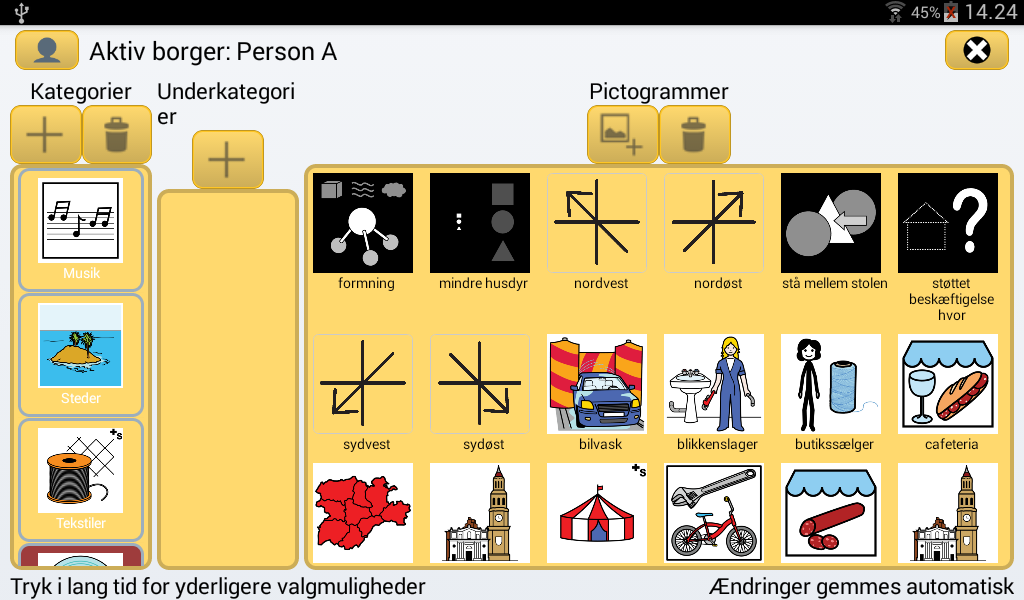
\includegraphics[width=\textwidth]{sprint_two/initial_category_tool}
    \caption{Old \ct}
    \label{fig:category_tool_old}
\end{figure}
% Indsæt billede af den nuværende skærm: .png

\subsection{Interaction design}

There is too much functionality on the same single screen in the current state of the \ct. Creation and modification of categories, sub-categories, adding and removing pictograms from categories is all done on the same screen which leaves little screen estate for each function.  

\subsubsection{Buttons}

The \ct includes non standardized buttons of different sizes and shapes. Buttons with square icons have different rectangular shapes. The buttons are too small in general and can be difficult to click. There is no margin between buttons which makes it easy to miss-click grouped buttons.   
% Alignment of buttons
The different buttons, and other widgets in general, in the \ct are not alligned very well

% Buttons popping in and out


\subsubsection{Android Design guidelines}

The Android design guidelines have changed and now advices to exclusively use long press action for multiple selection in lists. Long press is currently used to show a contextual menu for categories where it is possible to change the title, color, and icon of the category and to copy it. It is currently not possibly to perform multiple selection of pictograms. 

\subsubsection{Selection}

There is no visual cues of selection anywhere in the \ct. It is not possible to determine the currently selected category from the list of categories. This is a problem for the contextual delete button for categories. The contextual delete button for categories deletes the currently selected category but the only way to determine the current category is from the pictograms displayed to the right in the current selected category. 

\subsection{Crashes}

The application crashes when there are too many pictograms in a category and the user scrolls too far down in the list. 

\subsection{Explanatory text}

There 
% Not read
% Tells about hidden features

\subsection{Pop-ups windows}

% Popups in popups 
There is multiple contextual pop-ups in the application, for instance when creating a new category. Other pop-ups appears on top of the category creation pop-up when, for instance, the user neglects to provide a name when creating a new category. Pop-ups on pop-ups is not very good practice.  

% Popup overlay does not disappear 
There is another problem with the pop-ups. The pop-ups creates an overlay ontop of the remaining background

only this overlay does not disappear when they are closed using the Android soft- or hardware- back button instead of their cancel button.
 
\subsubsection{Monkey tests}

